% F089｜勾股整数数组的构造规律｜04_examples.tex
% 继承上传模板的 LaTeX 环境；当前条目的内容独立编写。
\clearpage
\begin{examplebox}
\textbf{\textcolor{CExample}{例 1：构造5,12,13}}
\par\medskip
\begin{center}
% F089｜formula 原创简明教学示意图
\begin{tikzpicture}[>=stealth,scale=.9]
\node[draw,rounded corners,fill=teal!9] (a) at (0,0) {$m>n>0$};
\node[draw,rounded corners,fill=orange!10] (b) at (4.5,0) {$m^2-n^2,\ 2mn,\ m^2+n^2$};
\draw[->,thick] (a)--(b);
\node at (4.5,-1){\small 任取正整数 $m>n$，都会得到一组勾股数};
\end{tikzpicture}

\end{center}
\medskip
取 $m=3,n=2$：$m^2-n^2=9-4=5$，$2mn=12$，$m^2+n^2=13$。所以 $5^2+12^2=13^2$。
\end{examplebox}
\clearpage
\begin{examplebox}
\textbf{\textcolor{CExample}{例 2：给出奇数9，马上得三边}}
\par\medskip
\begin{center}
% F089｜odd 原创简明教学示意图
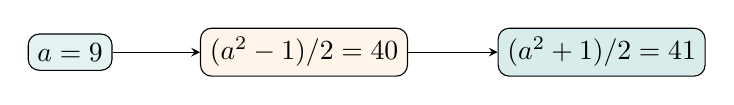
\begin{tikzpicture}[>=stealth,scale=.9]
\node[draw,fill=teal!10,rounded corners] (a) at (0,0){$a=9$};
\node[draw,fill=orange!8,rounded corners] (b) at (3.3,0){$(a^2-1)/2=40$};
\node[draw,fill=teal!15,rounded corners] (c) at (7.5,0){$(a^2+1)/2=41$};
\draw[->] (a)--(b);\draw[->] (b)--(c);
\end{tikzpicture}

\end{center}
\medskip
$a=9$，另外两边为 $(81-1)/2=40$ 和 $(81+1)/2=41$，得到 $\boxed{(9,40,41)}$。
\end{examplebox}
\clearpage
\begin{examplebox}
\textbf{\textcolor{CExample}{例 3：给出偶数10，马上得三边}}
\par\medskip
\begin{center}
% F089｜even 原创简明教学示意图
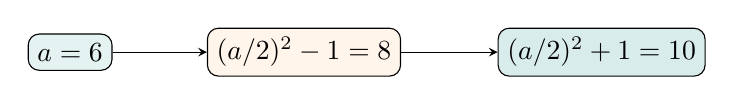
\begin{tikzpicture}[>=stealth,scale=.9]
\node[draw,fill=teal!10,rounded corners] (a) at (0,0){$a=6$};
\node[draw,fill=orange!8,rounded corners] (b) at (3.3,0){$(a/2)^2-1=8$};
\node[draw,fill=teal!15,rounded corners] (c) at (7.5,0){$(a/2)^2+1=10$};
\draw[->] (a)--(b);\draw[->] (b)--(c);
\end{tikzpicture}

\end{center}
\medskip
$a=10=2\times5$，另外两边 $25-1=24$、$25+1=26$，得到 $\boxed{(10,24,26)}$。
\end{examplebox}
